\documentclass[10pt,twocolumn]{article} 

% required packages for Oxy Comps style
\usepackage{oxycomps} % the main oxycomps style file
\usepackage{times} % use Times as the default font
\usepackage[style=numeric,sorting=nyt]{biblatex} % format the bibliography nicely

\usepackage{amsfonts} % provides many math symbols/fonts
\usepackage{listings} % provides the lstlisting environment
\usepackage{amssymb} % provides many math symbols/fonts
\usepackage{graphicx} % allows insertion of grpahics
\usepackage{hyperref} % creates links within the page and to URLs
\usepackage{url} % formats URLs properly
\usepackage{verbatim} % provides the comment environment
\usepackage{xpatch} % used to patch \textcite
\usepackage{graphicx}

\addbibresource{references.bib}
\DeclareNameAlias{default}{last-first}

\xpatchbibmacro{textcite}
  {\printnames{labelname}}
  {\printnames{labelname} (\printfield{year})}
  {}
  {}

\pdfinfo{
    /Title (Computational Queries: Discoverability and Curiosity in User Centered Design)
    /Author (Joaquín Madrid Larrañaga)
}

\title{Computational Queries: Discoverability and Curiosity in User Centered Design}

\author{Joaquín Madrid Larrañaga}
\affiliation{Occidental College}
\email{jmadridlarra@oxy.edu}

\begin{document}

\maketitle

\section{Introduction and Problem Context}
From interactive sculptures to light projections, the interactive art scene has captivated audiences throughout the world \cite{sarto_disneys_2021, noauthor_teamlab_2020}.  By creating digital projections, responsive animations, and live video feeds, artists have blurred the lines between traditional art and technology to create installations unlike any other.  Many of these installations incorporate visuals and audio and ask participants to interact with physical pieces of the exhibit. This interaction is usually tactile, verbal, or a motion on the part of the audience that causes a change in the art piece itself.  Through their interactive nature, these exhibits allow users to experience art in a 4D space since the exhibit changes with interactions over time. 

Since the 1960s, interactive art exhibits have enthralled artists and computer scientists alike \cite{trifonova_software_2008}.  While these initial installations were not computationally intensive, they still captured the imaginations and curiousities of users young and old.  However, it is important to ensure that appropriate instructions are given to the user regarding the intention of the project as well as the appropriate mode of interaction. \citetitle{hornecker_x201ci_2008} by \citeauthor{hornecker_x201ci_2008} examines a case study of an interactive installation at a science museum.  Users explained that the installation was ``busy'' and ``had a lot going on''.  As a result, it was unclear both how users were supposed to interact with the exhibit and what they were supposed to learn from the installation. When designed correctly, these cues remind the user of the intention of the project while also nudging them in the right direction for the next step in their user journey.  For the installation discussed in this paper, these types of ambiguity were avoided whenever possible. Additionally, two rounds of user testing were conducted to identify any unclear modes of gameplay in order to rectify them prior to large scale showcase. 

``Computational Queries'' is an interactive art installation that incorporates user movement and responsive projections to create geometric graphics that shift and change according to the position of a user's hands.  Users will wave their hands around in front of the camera and the geometric pattern will react in real time. Similar to a game, this installation has additional levels that users can achieve by completing certain tasks.  For example, if a user waves their hand across the screen, they may collect objects in their hand across the screen.  Once all the objects are collected, the next level will be initiated.  This new level will have a different type of interaction and a different task that must be completed to move on to the subsequent level.  After 4 levels, the installation will return back to the beginning.  As a result of this cyclical nature, users will be able to spend as little or as much time interacting with the installation as they would like since there is no true end or beginning. On the other hand, users may not even wish to move on to another level since they can interact and shift with any one level for as long as they would like.  

\begin{figure}[hbh]
\begin{center}
\scalebox{.5}{
\includegraphics{images/triangle_inspo.png}} 
\vspace{.5cm}
\caption{Image reference for the geometric design of level 2.}
\label{fig:geometric}
\end{center}
\end{figure} 

In order to increase variation for users who cycle through the installation many times, easter eggs will be implemented at several edge cases within each level.  For example, if a user places one hand on one side of the installation and the other hand at the other side a new color or feature may be displayed.  Users who spend more time will discover more easter eggs, but users who spend less time will still be able to interact with and enjoy the installation without feeling confused about how to operate the installation.  In order to aid with any confusion, there will be visual hints and motions to encourage user interaction. These hints will fade in after a certain amount of inactivity from the user, but will not interfere with user play if the user decides to explore one level instead of advancing. 

``Computational Queries'' seeks to explore the innate curiousity within each person as well as curated discoverability within any well-designed app and game. This exhibit aims to provide an avenue for exploration and accomplishment through play.The installation will allow users the flexibility to explore and discover new features and levels while also giving the users a sense of accomplishment when they discover something new even if it was not an advancement to the next level. As a whole, this installation intends to provide users with a carefree way to move their bodies, tap into their inner curiousity and problem solving skills, and enjoy a different mode of gameplay than they are used to. 


\section{Technical Background}
At the highest level, this installation focuses on human movement as the primary way of interacting with a computer.  This project will use handtrack.js, an open source hand tracking software developed by Victor Dibia \cite{noauthor_handtrackjs_nodate-1}, to interpret user movement as input for the computer.  This software will use the video feed from a webcam to indentify and classify human hands (of any configuration) and human faces.  This is done through a Region-based Convolutional Neural Network (RCNN). Each frame of the video feed is fed through the RCNN to produce bounding boxes aroun each instance of a face or hand (Figure \ref{fig:bounding_boxes}). The coordinates of these bounding boxes are extracted and used to track the position of users' hands throughout gameplay. 

\begin{figure}[hbh]
\begin{center}
\scalebox{.4}{\includegraphics{images/bounding_example_resized.png}} 
\vspace{.5cm}
\caption{Classification and bounding boxes for a frame of a person}
\label{fig:bounding_boxes}
\end{center}
\end{figure}

Handtrack.js also classifies each hand as ``open'', ``closed'', ``pinch'', or ``point''.   While this current implementation does not differentiate between different types of hand classification for gameplay, this capability provides a possibility for more nuanced interactions for additional levels or iterations of the installtion. Since handtrack.js is a JavaScript based package made for web applications, it makes sense to create this installation using HTML5, CSS3, JavaScript graphics, and a webcam - elements that interface well with many common browsers and computers.   As a result, this installation may be repurposed as a web application for the general public after its run as an installation at Occidental College. 

Initial testing of handtrack.js revealed that it has a very small number of frames per second (FPS) that varies between 8FPS and 16FPS.  This fluctuation is based on how fast the recognition software can process each frame of the video input. More processing time = less frames outputted.  Fortunately, this is not a sequential delay in output (the cause of lag, also called first in, first out), but rather a first in, last out approach.  In this way, any frames that were missed as a result of the processing time are discarded and the next newest frame is processed.  Even though this approach does not interfere with continuity for the viewer, it produces a jerky video as a result of the reduction in FPS.  

The industry standard for high definition films is 24 FPS \cite{noauthor_3_nodate} which is the smallest number of FPS that creates smooth motion.  The proposed implementation of handtrack.js produces almost half of the industry standard which causes a jerky live video feed.  Fortunately, the individual bounding boxes create convincing continuous motion when the live video feed is removed and only the bounding boxes remain. In the final installation, these bounding boxes will also be removed and the movement of the pattern will cue the user in to where their hand is positioned in relation to the installation.  

Unfortunately, user motion needs to be fairly slow in order for the program to accurately identify the user's hands.  Since faster motion causes motion blur in photos, each individual frame will be blurred if the user moves quickly. As a result, the image recognition software is unable to correctly identify the bounding boxes of the hands since their shape is blurred. Further research suggests that an easy solution is to reduce the exposure time for each individual frame which will remove the blur \cite{e_adjusting_2019} and allow for better hand recognition.   

While all of these solutions could have been implemented, most of these problems were solved with a more powerful computer.  Instead of using the HP computer with 8 GB of RAM, an MSI laptop with 16GB of RAM was used for the final presentation of the project.  This compter offered between 20-30 FPS for the live vdieo feed. 

This project will also make use of the ``Model, View, Controller'' (MVC) architecture often used in games.  This modl details the way these three components interface with each other. In the MVC architecture, the user interfaces with the controller which sends information to the model.  The model then changes according to the controller and updates the view which the user observes.  Based on this update, the user will decide what action to take through the controller to continue the cycle. 

The model will be written in JavaScript and will interface with handtrack.js (the controller) and the view (the HTML output).  The view will be generated using the built in JavaScript canvas properties to create geometric patterns that shift and change according to user movements. 

\section{Prior Work}

\citetitle{kwon_real-time_nodate} by \citeauthor{kwon_real-time_nodate} highlights many interactive generative art exhibits from the early 2000s. In 2002, Scott Snibbe created a visualization that recorded users' shadows and played them back allowing the user to add new shadows to the playback loop - similar to a guitar feedback loop (Figure \ref{fig:shadow-2002}).  In much the same way, ``Computational Queries'' offers ever-changing and growing graphics to add interest over time.  

\begin{figure}[hbh]
\begin{center}
\scalebox{.12}{\includegraphics{images/shadow-2002.jpeg}} 
\vspace{.5cm}
\caption{A person watching Scott Snibbe's ``Shadow''. }
\label{fig:shadow-2002}
\end{center}
\end{figure} 

Then, in 2015, Philip Worthington created the installation ``Shadow Monsters`` which used machine learning to recognize specific shapes and features in a user's shadow and modify it too create a `monster' \cite{houston_public_media_mfah_2015}.  For example, shadows that look like circles will be made into the monster's eyes, and shadows that look like intersecting lines will be made into the monster's mouth.  This transformation happens in real time and artificial extremeties are added in real time to the user's shadow.  This installation offers an exciting experience for users of all ages, a consideration that was also taken for ``Computational Queries''.  However, ``Shadow Monsters'' offers only one style of gameplay, albeit a highly engaging one.  However, for users who are intent in pushing the limits of the installation and figuring out what inputs produce the desired outputs, there is a finite solution.  ``Computation Queries'' seeks to increase engagement for these types of curious users through it's multi-level approach. 

``Future You`` (2019) by Universal Everything, a technological art company, focuses on real time mirroring of the user to animate a unique CGI character \cite{noauthor_future_2019}. This CGI character is a humanoid, futuristic being that is unique for each user based upon predetermined variables. Additionally, this character undergoes an evolution every 5 seconds becoming more complex the longer a user interacts with it.  In this way, the program is generating and modifying the art based upon the user's actions according to various variables (time and appearance).  Users of ``Future You'' are naturally curious to discover the extent to which the character mimics thier movements and often tried to push the limits of this installtion.  This type of user interaction is heavily anticipated and encouraged for ``Computational Queries''. 

``Computational Queries'' draws a lot of inspiration from Aakash Nihilani, an artist known for his 3D geometric illusions. Specifically, his interactive geometric series titled ``Projections'' from 2015 \cite{noauthor_aakash_nodate}.  These interactive projections incorporate different geometric patterns that flow and ebb as users run their hands along the wall that the projections are screened on (Figure \ref{fig:squares}). As these geometric patterns move, bright colors are revealed in the space between each shape.  Nihilani strives for simplicity and minimalism in all of his artwork.  As a result, the movement in each of the installations in ``Projections'' is contained and easily learned.  ``Projections'' offers an opposite challenge to users than ``Future You''.  Users of ``Future You'' are curious to learn about the installation because it is potentially complicated and evolves new and interesting features over time.  In contrast, ``Projections'' is deceptively simple which prompts users to spend time testing the simplicity and trying edge cases in order to produce something new and interesting... to no avail. Though one could argue that this humanistic testing of the exhibit is interesting and fun for the user.

In this way, ``Computational Queries'' draws inspiration from all of these previous works while also building upon and improving features of each to highlight the themes of curiousity and discoverability within the installation. 

\begin{figure}
\begin{center}
\scalebox{.35}{\includegraphics{images/squares-2015.png}} 
\vspace{.5cm}
\caption{A person interacting with Aakash Nihilani's ``Squares''. }
\label{fig:squares}
\end{center}
\end{figure} 

\section{Methods}
 A tutorial by Larry Sass-Ainsworth on medium.com \cite{sass-ainsworth_getting_2019} provides a starting point for a functional version of handtrack.js.  This tutorial covers how to add handtrack.js to any HTML project and provids source code for a intuitive video feed that tracks face and hand positions. After following this tutorial, the JavaScript code was edited to remove the live video feed and graphics were added using the JavaScript canvas feature.  These graphics consisted of a large circle that moved when it was touched by the handtrack.js bounding boxes.  As a result, a user was able to push the large circle around the screen. 
 
 
\subsection{Design: Feelings and User Consideration}
 When designing the overall feel of the installation, it was important to the artist that there was no connection to the physical world.  The installation was meant to convey a serene, abstract space reminiscent of exploring the unknown.  As a result, simple shapes and colors were chosen to make up the building blocks of each world. While this abstract design offers a large realm of possibilities, the shapes still obey Newtonian physics as they move around the screen.    
 
 Initially, this installation was created with three different types of users in mind:
 \begin{enumerate}
  \item Fast users
  \item Slow users
  \item Watchers
\end{enumerate}
  As a large scale interactive installation, there will be people who are unimpressed or easily bored with the installation.  These users will likely move their hands quickly across the screen and are eager to move on to the next portion of the exhibit. As a result, the first level offered a feature where users were rewarded for moving circles quickly across the screen and could actually move on to the second level by moving all the circles fast enough.  However, Handtrack.js has trouble classifying hands that are moving fast...an issue that is discussed in more detail later. 
 
  ``Slow users'' are users that tend to move slow and methodically.  They are interested in testing each portion of the level and discovering what is possible within the installation. These are the users that will push the edges of the capabilities of the installation. 
 
  ``Watchers'' are users who do not interact with the installation itself. These could be parents who bring their children, differently abled users who cannot interact, or people who just prefer watching to interacting. These users guided many of the color schemes, dazzling moving elements, and future sound choices. 
 
 \subsection{Foundational Level Structure}
To structure the abstract nature of the graphics, a framework consisting of six fundamental rules to govern all the levels was created.  These rules are largely based upon Mihaly Csikszentmihalyi's concept of flow \cite{csikszentmihalyi_flow_1990} and consist of the following:
\begin{enumerate}
  \item The contents of the screen must move regardless of interaction.
  \item When someone enters the space, the contents of the screen must react in some way.
  \item Each level must have a distinct goal for the user to strive towards.
  \item There must be some sort of indication or feedback that the user is advancing towards completing the goal.
  \item There must be some sort of indication that the user has completed the goal. 
  \item There must be a seamless transition to the next level.
\end{enumerate}

These rules are intended to facilitate flow while also unifying the levels into a cohesive project.  The initial movement required by the first rule is intented to draw the viewers attention towards the installation and to offer visual excitement in the absence of interaction.  The second rule nudges the user towards the possibilty of interaction by notifying them that the installation will respond with user input. The third rule acts as an incentive for the user to continue interacting with the installation. While not immediately obvious, this foundational feature offers consistancy between the levels as users learn to interact and try to discover what the goal of the level is. As a basic UI principle, feedback is thoroughly necessary to let the user know that they are completing some aspect.  Rule four explicitly requires feedback for each level. Rule five acts as an extension of rule four. Rule six ensures that the user cognatively retains information they learned in the previous level.  By creating transitions that morph and change one level into another, it is clear that the level is in the same world as the previous one, cluing the user into the fact that the levels will behave similarly.  It is now up to the user to discover the differences. 

\subsection{Level One}

\begin{figure}[hbh]
\begin{center}
\scalebox{.4}{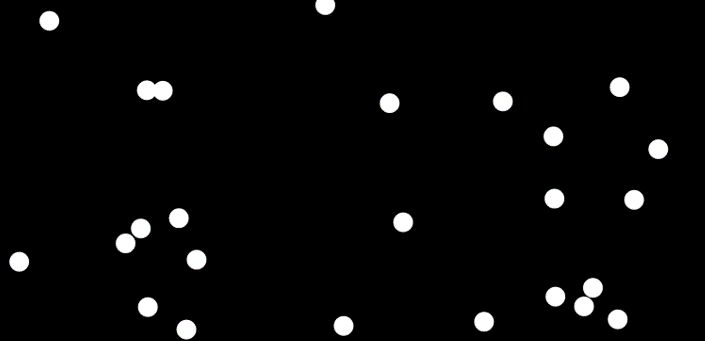
\includegraphics{images/white_circles.png}} 
\vspace{.5cm}
\caption{Prior to a user entering the space, the circles float around the screen and bounce off the edges of the canvas.}
\label{fig:white_circles}
\end{center}
\end{figure} 

Largely inspired by celestial objects, the first level features 40 white circles bouncing around the screen (Figure \ref{fig:white_circles}).  The goal of level one is to collect all the circles into a user's hands. When a user's hand is detected, the circles oscillate between positive and negative motion creating a jittering effect.  If circles are close to a user's hand, they move towards the hand, gaining speed as they move closer.  However, if a circle moves past a user's hand due to its high velocity, it quickly changes direction.  This behavior simulates the gravitational pull of the user's hand on the circles.  When the circles are close to the user's hand, they change color to encourage the user to collect all the circles (Figure \ref{fig:green_circles}). As the user collects more and more circles, they overlap into one circle that is in the middle of the user's hand. If the user leaves the installation or drops their hand, these circles will disperse across the screen once again.  Once all the circles have been collected, they change color once again and shoot across the screen (Figure \ref{fig:red_circles}).  This signifies the completion of the goal.  

\begin{figure}[hbh]
\begin{center}
\scalebox{.4}{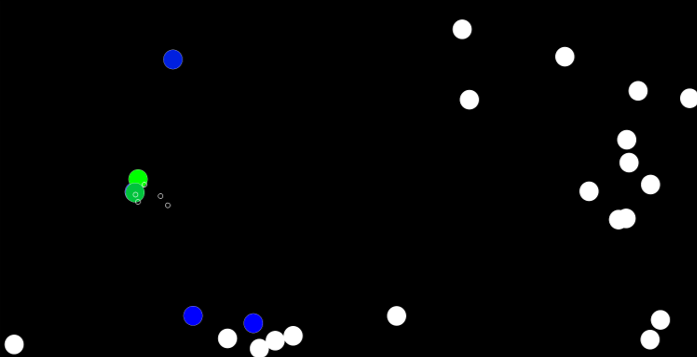
\includegraphics{images/green_circles.png}} 
\vspace{.5cm}
\caption{If a circle is close to the user's hand, it turns blue. The faster a circle is moving as it gets closer to the hand, the greener it turns.}
\label{fig:green_circles}
\end{center}
\end{figure} 

\begin{figure}[hbh]
\begin{center}
\scalebox{.4}{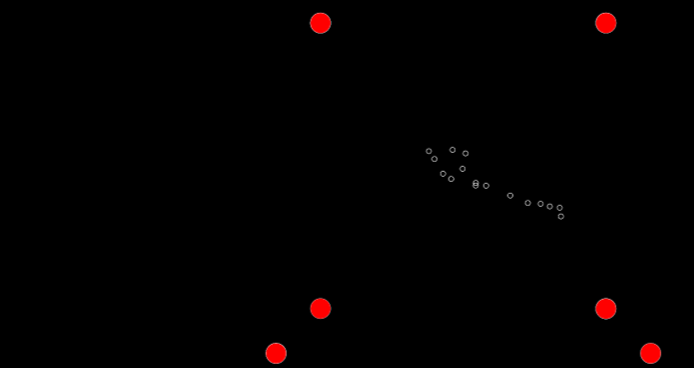
\includegraphics{images/red_circles.png}} 
\vspace{.5cm}
\caption{Once a user has collected all the circles they turn red and shoot off the edge of the screen.}
\label{fig:red_circles}
\end{center}
\end{figure} 

Originally, the white circles turned blue if they were close to the user's hand and then faded into green the faster they moved.  This was to encourage users to move their hands fast while dragging a circle that was caught in the gravitational pull of the user's hand. If the user was able to get a circle to move fast enough, it changed color again and flew off the screen.  This was another was to succeed in the level: drag each circle, or a collection of circles, fast enough so that they change colors and shoot off the screen instead of bouncing back.  However, because of motion blur, the handtracking software struggles to recognize hands that are moving fast.  As a result, users were unable to complete this task during user testing trials. In addition, many users were unaware that this was a functionality and didn't explore it.  

\subsection{Level Two}

\begin{figure}[hbh]
\begin{center}
\scalebox{.4}{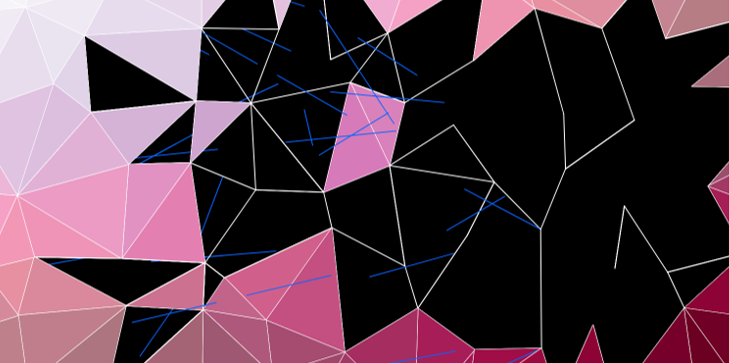
\includegraphics{images/middle_tri.png}} 
\vspace{.5cm}
\caption{Lines shoot across the screen and when a user touches a line, it freezes in its place creating an intersection of triangles.}
\label{fig:middle_tri}
\end{center}
\end{figure} 

Level two focuses on a lattice of triangles.  This lattice is generated by Trianglify, a javacript library written by Quinn Rohlf \cite{rohlf_trianglify_2022}.  Each triangle making up the lattice is separated into the edges that make up the three sides.  These edges move across the screen according to their slope.  When a line is touching its position as an edge of a triangle and it is being touched by the user, it will lock its position on the screen (Figure \ref{fig:middle_tri}).  Once all three sides of a triangle has been locked, the triangle will be colored in according to the colors generated by Trianglify. Since Trianglify easily generates different lattices, a new lattice is generated each time level two is played.  This is intentional to capture the interest of users who may be interacting with levels multiple times.   

\section{Evaluation Metrics}
\citetitle{bernhaupt_video_2010} by \citeauthor{bernhaupt_video_2010} suggests that user testing should be done at every stage of development and provides a framework for different types of testing: free flow, narrow specific, and broad specific.  This project focused on the concept of free flow. Free flow allows users to explore the exhibit at will and play as long as they are interested.  This provides a useful time based metric that will quantifiably express how interested users are.  Furthermore, this approach will highlight any portions of interaction that are unclear or confusing to users as they experience it in real time. 

Prior to testing the installation, users were asked to complete a survey that assessed their previous knowledge with similar modes of gameplay and user interaction.  Both the survey and the raw results of the survey can be found in the Github repository for this project.  These questions focused on controllers such as xBox, Wii, and xBox Kinect. Then the users were randomly assigned a level to start on; one or two.  Users were asked to narrate their actions and discuss why they were making the decisions they were.  They were also notified that the researcher may ask follow up questions during or after the testing of the installation. Due to time constraints, the first round of user testing was completed while the second level was still in development.  Users were allowed to complete the testing alone or with a partner.  One instance of user testing was conducted with three users. 

During this time, the researcher noted how much time was spent on each level, interesting quotes from users, bugs discovered in the functionality, suggestions for improvement, and if the users completed the level.  If the user was unable to finish a level and expressed boredom or interest in moving to the next portion of testing, the level was manually changed. 

After completing both levels, users were asked to take a followup survey which focused on user experience.  This portion asked users to list emotions they were feeling and asked them to contemplate specific goals of the project relating to flow.  Additional questions in this section such as ``I developed a clear objective as I was playing each level of the exhibit.'' and ``I would enjoy watching other people interact even if I wasn't the person interacting.'' were asked in likart scale form. 

During the second round of user testing, the same procedure was performed. A successful completion of this installation would be marked by strong (but not necessarily positive) emotions elicited in users, an indication of visual interest in the exhibit, a clear understanding of the functionality of the exhibit, and a desire to determine and complete the goal of each level.  

\section{Results and Discussion}
After the first round of user testing, several bugs were discovered and swiftly repaired:
\begin{enumerate}
  \item A miscalculation when counting the number of circles collected by a user in level one.
  \item The circles stayed clumped together when a user dropped their hand instead of dispersing. 
  \item When a user is not moving their hand very fast, some circles are not moving towards the hand, but instead are frozen, despite the fact that they changed color indicating that they should be moving towards the hand. 
  \item Lines with steeper slopes moved too fast for users in level two. 
\end{enumerate}

Round one of user testing produced many statements similar to ``I don't understand'', ``I'm confused'', and ``I don't know how I did that''.  Furthermore, many users listed emotions such as frustration, anger, and confusion. Several users also indicated that the installation did a bad job of clarifying when it detected them in frame and when it did not. 

As a result, a visual representation of the user's hand on the screen was added.  Initially, there was no representation or ``shadow avatar'' of the user in the installation itself. As a result, users were unable to tell where their hands were with relation to the objects on the screen.  As a result, it was difficult for users to determine if they were interacting and colliding with objects correctly. In order to rectify this, small hollow circles were added to represent the user's hands. However, it was at this point that the researcher discovered that the handtracking software sometimes failed to recognize hands for several frames before re-recognizing a hand that hadn't moved.  As a result, the computer had no way of knowing that these two bounding boxes were classifying the same user's hand, but instead treated them as different hand instances.  This caused large difficulty for users in level one. Because circles were attracted to the bounding boxes, if the software failed to classify the hands for several frames, the circles changed colors back to white and moved away from the hands at no fault of the user.  In order to recitfy this issue, a heuristic was developed to determine if new bounding boxes were related to bounding boxes in previous frames and were therefore likely the same hand.  Then, each bounding box was represented on screen for 24 frames in the event that the handtrack software failed to recognize a hand.  Then, if no new instances of the same hand were detected, the bounding box was erased. 

While the second level was not functioning as intended during the first round of user testing, it was still useful to see how users expected to be able to interact.  During this testing, the lines criss-crossed across the screen, but the collision that caused lines to freeze was not working properly and only worked part of the time.  However, even when lines did freeze, users did not notice, likely because there was no visible change except for a stop of motion. And even when lines did freeze, users still did not make it far enough in the level to realize that they were building triangles.  As a result, triangles along the edges were added to clue the user into the fact that they are building additional triangles. 

The second round of user testing featured all of the above changes as well as a functional second level.  The results of the second round produced much more language similar to awe, entertainment, and curiosity. In addition, users commonly said ``we did it!'' and ``that was really fun''.  These suggest a sense of accomplishment at completing the level and a level of satisfaction with their accomplishment. 

\begin{figure}[hbh]
\begin{center}
\scalebox{.6}{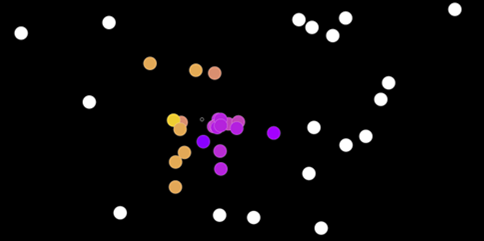
\includegraphics{images/newcolor1.png}} 
\vspace{.5cm}
\caption{A new color scheme for level two.}
\label{fig:newcolor1}
\end{center}
\end{figure} 

During the second round of user testing, one user commented that they were surprised that the circles in level one changed color to red when the user completed the level since they do not associate red with success.  This prompted a reexamination of the different colors used in both levels. Initially the circles turned blue when interacted with, turned green when they moved fast, and red when the level was completed (Figure \ref{fig:newcolor1}). After recoloring, the circles turned purple when interacted with, yellow when moved fast, and green when the level was completed. This was to emulate the color scheme of galaxies and to associate green with success.  

\begin{figure}[hbh]
\begin{center}
\scalebox{.6}{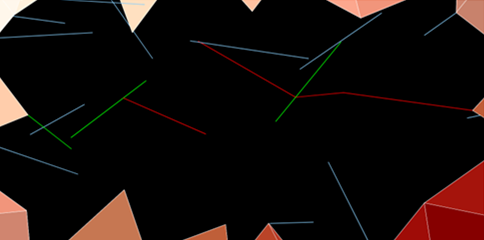
\includegraphics{images/newcolor2.png}} 
\vspace{.5cm}
\caption{New color indicators for level two.}
\label{fig:newcolor2}
\end{center}
\end{figure} 

In a similar vein, the colors of the lines in level two were also changed.  When a line is able to be frozen by the user through collision, it turns green, otherwise it is white. If the line has collided with a user and is in the process of freezing, it turns blue (Figure \ref{fig:newcolor2}).  It was clear that users didn't know that they had succeeded in freezing a line until it was frozen and since a line can be frozen before it reaches its final position, users needed immediate feedback when they succeeded in freezing. When a line is frozen post-collision, it turns red to draw attention to newly frozen lines.  During user testing, users did not notice that any lines were freezing for an extended period of time. 

During unofficial testing, these color changes seemed to aid in user understanding, though the exact mechanics for the second level seemed to escape the majority of users who interacted with the exhibit. More development needs to be done to finetune the collision of the lines with the hands as well as to highlight overall user success with regards to rule four. 

As a whole, based upon the results of the survey,  users developed clear objectives during the levels, were able to understand when/if the installation detected them, and enjoyed watching the exhibit when they were not interacting. These findings suggest that the installation met its goals of eliciting strong emotions (most commonly awe, frustration, and happiness), visual interest in the exhibit, an understanding of the functionality of the installation, and a strong desire to determine and complete the goals of each level. 

\section{Ethical Considerations}

\subsection{Ethical Design}\label{sec:design}

In the textbook ``Introduction to Art: Design, Context, and Meaning,'' \cite{blood_introduction_nodate}the authors caution against different types of unethical practices when creating an art piece. \citeauthor{blood_introduction_nodate} warns against `appropriation' or the act of incorporating another artist's work into their own without any change or edits and without acknowledgement or credit. Similar to plagarism, this type of artistic appropriation not only steals intellectual property from the original artist, but also damages the credibility of the emerging artist.  While artists often borrow ideas, aesthetics, or even entire pieces from other artists, ``Introduction to Art: Design, Context, and Meaning'' makes the distinction that these artists are intentionally altering the original idea in order to comment on it's original meaning or to recontextualize it in a new setting. In this way, new artists are still bringing their own intentions and ideas to the original work.  

As mentioned above, this project draws a lot of inspiration from Aakash Nihilani.  While Nihilani's projection work focuses on interactive geometric works,``Computational Queries'' will ask users to wave their hands in front of geometric patterns in order to reveal another `level' of the game.  Even though ``Computational Queries'' will have a different color scheme and type of user interaction than ``Projections,'' the two installations are still very similar in structure and topic.  As such, the final installation will offer a special thanks or acknowledgement for Aakash Nihilani as an inspiration for this work. 

\subsection{Ethical Interaction}\label{sec:interaction}

As mentioned, this installation focuses on human movement as input.  Unfortunately, not all users will be able to interact with the installation.  Hand amputees will not be able to advance to the next level or cause changes to the installation since the hand tracking software will not be able to accurately capture their arm movements. Furthermore, users with motor inhibitions may not be able to accurately complete the motions needed to advance to the next level.  These motions could include moving hands from side to side, or bringing hands together and apart again; motions that are not possible for every user. 

Providing additional ways to interact with the piece becomes integral when dealing with differently abled people. For example, a joystick controller, handheld mouse, or eye tracking software as inputs to determine the position of the movement allows differently abled people alternative ways to interact that don't involve their hands. This type of interaction is necessary to advance through the installation, however, differently abled people will still be able to experience the installation by watching someone else interact in real time.

This installation relies heavily on visual feedback for the user.  Users are visually instructed how to interact with the exhibit and then, when they are interacting, the installation responds to their movements by visually updating the displayed projection.  Furthermore, people who interact with the exhibit will be visually prompted with hints on screen as well as given visual feedback as a metric for success through the levels. As such, users with visual impairments will not experience any sensory differences as they physically interact with the installation.  For all intents and purposes, they will have walked into an empty room and nothing will signal that anything has changed. 

In order to account for this, a compelling soundscape that changes as a user interacts can mimic the visual outputs aurally. For example, as the user interacts with the pattern by moving their hands, the music could change or add a sound.  In this way, blind and low vision users can still interact with the exhibit. Furthermore, these sounds could also move to different speakers throughout the room, a technique that could motivate blind/low vision people to move around the space which would further change the audio landscape.  

\section{Conclusion}
``Computational Queries'' seeks to motivate users to tap into their inner curiousity and experience an abstract art piece by moving their body.  Through common UI principles, such as shape, color, and movement, the installation seeks to inform users of the possibilities and the goals of the levels while also leaving room for the user to discover features on their own. This paper discusses the functions of the first two levels as preparation for the full scale projection installation.  In the future, two more levels will be created that incorporate more involved movements on the part of the user (tasks that require both hands) and improved graphics (particle generations and gradients). Furthermore, considerations such as camera placement, projector type, speaker placement, audio creation and mixing, and installation location will be investigated.  Lastly, the considerations  discussed above for differently abled people will be implemented and tested.  After these steps, the projection hopes to be installed on campus at Occidental College as a full scale interactive art installation.  

\printbibliography 

\end{document}
